\documentclass[11pt]{article}
\usepackage{geometry}                
\geometry{letterpaper}                 
\usepackage[parfill]{parskip}        
\usepackage{graphicx}
\usepackage{amssymb}
\usepackage{amsmath}
\usepackage{courier}
\usepackage{epstopdf}
\usepackage{verbatim}
\usepackage{float}
\usepackage{enumerate}
\usepackage{hyperref}
\usepackage[utf8]{inputenc}
\usepackage[T1]{fontenc}
\DeclareGraphicsRule{.tif}{png}{.png}{`convert #1 `dirname #1`/`basename #1 .tif`.png}
\usepackage{color}
\usepackage{textcomp}
\definecolor{listinggray}{gray}{0.9}
\definecolor{lbcolor}{rgb}{1,1,1}

\begin{document}
{\small
\section*{Problems for Discussion 8, 11/12/13}
Compiled by Mai Le, some problems from Prof. Fessler
}

\section{DFT properties}
% Fessler exam 3 of Winter 2004, number 6
Determine the output of the following Matlab command: 

\texttt{fft(fft([3 4 5 6]))}

{\color{blue}
In Matlab, if you call \texttt{fft(x,n)}, it will perform the \texttt{n}-point DFT of \texttt{x}. However, if you do not supply a second argument- \texttt{fft(x)}, Matlab will find the length of \texttt{x} and use that for the length of the DFT. So this command applies a 4-point DFT to $x[n] = \{\underline{3}, 4, 5, 6\}$ twice.

From duality, we know that the output will then be $y[n] = 4x[-n\ mod\ 4]$. The circular time reversal results in $\{\underline{3}, 6, 5, 4\}$, so $y[n] = \{\underline{12}, 24, 20, 16\}$ or \texttt{[12 24 20 15]}.
}

% and number 7
Determine the output of the following Matlab command:

\texttt{ifft(fft([1 2 3 0 0 0].*fft([1 0 1 0 0 0]))}

{\color{blue}
In general, this would be the 6-point circular convolution of the two signals, but there is adequate zero padding, so the circular convolution is the same as the linear convolution: \texttt{[1 2 4 2 3 0]}.
}

\section{Rational Rate Conversion}
% Fessler exam 3 of Winter 2004, number 8 and 9
A signal $x_a(t)$ was sampled at rate $F_1 = 30$ kHz and its samples $x_1[n]$ were stored. Later it is decided to recover this signal using an D/A converter that works at the sampling rate $F_2 = 20$ kHz. The following system has been proposed for solving this sampling rate conversion problem.

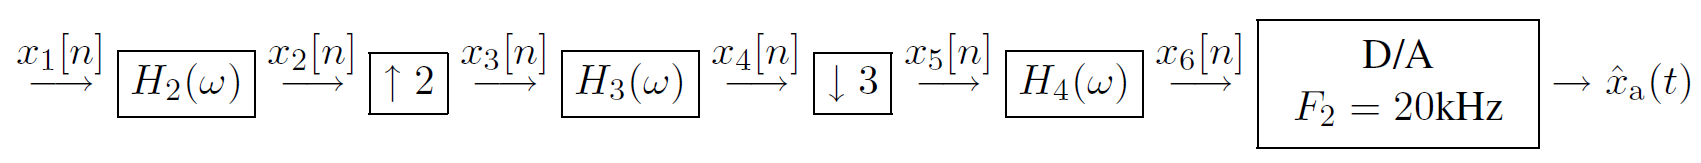
\includegraphics[width = 0.9\textwidth]{rate_conv_a.png} 

\begin{description}
	\item[(a)] Specify the magnitude responses of the three filters $H_2(\omega)$, $H_3(\omega)$, $H_4(\omega)$ so that the final output signal will be as close to the original signal as possible. If a filter is not needed, say so.
	\item[(b)] The following alternative system for solving the preceding rate conversion problem has also been proposed. Explain why this system would be (1) preferable, (2) inferior, or (3) equivalent to the system proposed in part (a).
	
	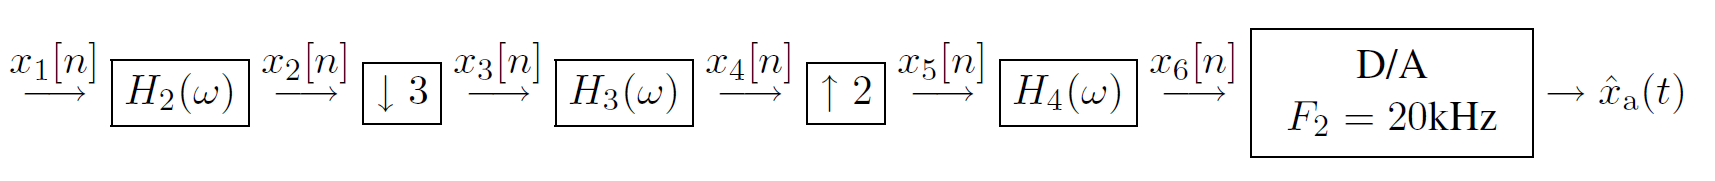
\includegraphics[width = 0.9\textwidth]{rate_conv_b.png} 	
\end{description}

{\color{blue}
This requires a lot of drawing, so I'll scan my drawings and upload them soon. In the meantime, this was covered in both sections, so you should be able to refer to your notes.
}

\section{DFT lengths}
% Fessler exam 3, Fall 1998, problem 1b

Suppose $x[n]$ is time-limited to $n=0,1, 2, 3$ and the 8-point DFT of $x[n]$ is given by

\[ \{\underline{5}, 3-j\sqrt{2}, 3, 3-j\sqrt{2}, 1, 3+j\sqrt{2}, 3, 3+j\sqrt{2} \} \]

Find the 4-point DFT of $x[n]$.

{\color{blue}
$\{\underline{5},3,1,3\}$
}

\section{DFT from the DTFT}
% Fessler exam 3, Fall 1998, problem 2a

A signal $x[n]$ has DTFT $X(\omega) = 4e^{-j13 \omega} + 3e^{j2\omega} + 2e^{-j11\omega}+7$. Find the 11-point inverse DFT of $\{X(\omega)\big|_{\omega = 2 \pi k /11}, k = 0,\ldots, 10\}$.

{\color{blue}
Let us first find $x[n]$. From linearity of the IDTFT and DTFT pairs, we can quickly see that $x[n] = 3 \delta[n+2]+t\delta[n]+2\delta[n-11]+4\delta[n-13]$. So the 11-point IDFT of the 11-point DFT is $\tilde{x}[n]$ with a period of 11. So we see that the points overlap as follows:

\[x_p[n] = x[n\text{ mod } 11] = \{\underline{9},0,4,0,0,0,0,0,0,3,0\} \]
}

\section{Uncertainty Principle}

For a signal $x[n]$ and its N-point DFT $X[k]$, 

\[ |support(x)||support(X)| \leq N \]

where the support of a signal is defined as:

\[ support(x)=\{n, x[n] \neq 0\},\ |support(x)| = \text{ number of elements in } support(x) \]

{\color{blue}
Proof: Coming soon...
}

%\newpage
%Berk's problem
%
%\[
%\begin{bmatrix}
%b & \underline{a}' \\
%\underline{a} & X 
%\end{bmatrix} \begin{bmatrix} w \\ \underline{v} \end{bmatrix} = 
%w \begin{bmatrix} b \\ \underline{a} \end{bmatrix} + \sum_{i=1}^n v_{i} \begin{bmatrix} a_i \\ \underline{x}_i \end{bmatrix} = 
%w \begin{bmatrix} b \\ \underline{a} \end{bmatrix} + \begin{bmatrix} \sum_{i=1}^n v_{i} a_i \\ \sum_{i=1}^n v_{i} \underline{x}_i \end{bmatrix} = 
%w \begin{bmatrix} b \\ \underline{a} \end{bmatrix} + \begin{bmatrix} \underline{a}'\underline{v} \\ X\underline{v} \end{bmatrix} =
%\begin{bmatrix} w b + \underline{a}'\underline{v} \\ w\underline{a}+ X \underline{v} \end{bmatrix} = 
%\lambda \begin{bmatrix} w \\ \underline{v} \end{bmatrix}
%\]
%
%\begin{align*}
%w b + \underline{a}'\underline{v} &= \lambda w\\
%(b-\lambda)w &= - \underline{a}'\underline{v} 
%\end{align*}
%
%\begin{align*}
%w\underline{a}+ X \underline{v} &= \lambda \underline{v} \\
%(X-\lambda I) \underline{v} &= w \underline{a} \\
%(X-\lambda I) \underline{v} &= - \frac{\underline{a}'\underline{v}}{b-\lambda}  \underline{a}
%\end{align*}
%
%If $\underline{a}'\underline{v} = 0$, then $\{\underline{v},\lambda\}$ is a eigen pair for $X$.
%
%If $\underline{v}$ is an eigenvector of $X$ with eigenvalue $\beta$ and $\underline{a} = \underline{v}$, then 

\end{document}